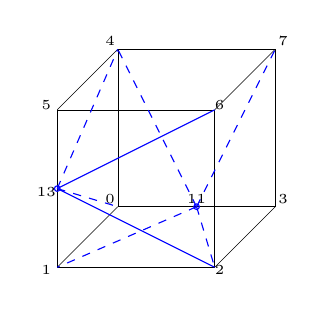
\begin{tikzpicture} %pattern4
		[cube/.style={very thin,black}]
	%draw the top and bottom of the cube
	\draw[cube] (0,0,0) node at (-0.1,0.1,0) {\tiny 0} -- 
                    (0,2,0) node at (-0.1,2.1,0) {\tiny 4} -- 
                    (2,2,0) node at (2.1,2.1,0)  {\tiny 7} -- 
                    (2,0,0) node at (2.1,0.1,0)  {\tiny 3} -- 
                    cycle;
	\draw[cube] (0,0,2) node at (-0.1,0,2.1) {\tiny 1} -- 
                    (0,2,2) node at (-0.1,2.1,2.1) {\tiny 5} -- 
                    (2,2,2) node at (2.1,2.1,2.1) {\tiny 6} -- 
                    (2,0,2) node at (2.1,0,2.1) {\tiny 2} -- cycle;
	
	%draw the edges of the cube
	\draw[cube] (0,0,0) -- (0,0,2);
	\draw[cube] (0,2,0) -- (0,2,2);
	\draw[cube] (2,0,0) -- (2,0,2);
	\draw[cube] (2,2,0) -- (2,2,2);

        \draw node at (1,0.1,0) {\tiny 11};
        \draw node at (-0.1,1,2.1) {\tiny 13};
        \draw[blue] (1,0,0) circle(1pt);
        \draw[blue] (0,1,2) circle(1pt);

        \draw[dashed,blue] (1,0,0)  -- (0,0,2);
        \draw[dashed,blue] (1,0,0)  -- (2,0,2);
        \draw[dashed,blue] (1,0,0)  -- (0,2,0);
        \draw[dashed,blue] (1,0,0)  -- (2,2,0);
        \draw[dashed,blue] (0,1,2)  -- (0,2,0);
        \draw[dashed,blue] (0,1,2)  -- (0,0,0);
        \draw[blue] (0,1,2)  -- (2,2,2);
        \draw[blue] (0,1,2)  -- (2,0,2);
\end{tikzpicture}
